\chapter{Introduction}

\textit{Vidjil} est une plateforme open-source \cite{giraudFastMulticlonalClusterization2014b}
permettant l'analyse de données de séquençage à haut débit pour l'étude du répertoire des gènes \gls{vdj} des 
cellules lymphoïdes. Ce processus de recombinaison somatique se produit au sein des précurseurs
B et T lors de la lymphopoïèse, et permet de générer un vaste répertoire d'anticorps et de récepteurs,
capables à leur tour de reconnaître une grande variété d'antigènes \cite{jonesTamingTransposonVDJ2004}.

\section{Répertoire des gènes \gls{vdj}}

Ce processus de recombinaison est complexe, et implique plusieurs étapes successives de réarrangement des segments
\gls{vdj} au sein des loci des \glspl{ig} et des \glspl{tcr} \cite{rothVDJRecombinationMechanism2014}.
Il débute par la sélection aléatoire de segments D et J, suivie de la sélection d'un segment V, au sein des chaînes
dites « lourdes », sous l'action des recombinases \gls{vdj}. Un mécanisme identique est observé pour les chaînes « légères »,
avec une recombinaison directe des segments V et J, sans étape D. À la suite de chaque recombinaison, des régions de diversité N 
de quelques nucléotides sont insérées aléatoirement entre les segments, contribuant à la diversité potentielle du répertoire 
(\autoref{fig:vdj}).

\vspace{1em}

Par conséquent, si l'on considère les loci des \glspl{ig}, la recombinaison \gls{vdj} permet de générer théoriquement : 

\begin{equation}
    \label{eq:combinaisons}
    \begin{aligned}
    \text{Chaîne lourde : } & \underbrace{50}_{\text{\# VH}} \times \underbrace{30}_{\text{\# DH}} \times \underbrace{6}_{\text{\# JH}} = 9000 \\
    \text{Chaîne légère } \kappa : & \underbrace{40}_{\text{\# Vk}} \times \underbrace{5}_{\text{\# Jk}} = 200 \\
    \text{Chaîne légère } \lambda : & \underbrace{46}_{\text{\# Vl}} \times \underbrace{7}_{\text{\# Jl}} = 322 \\
    \text{Total des combinaisons possibles : } & 9000 \times (200 + 322) = 4\,698\,000
    \end{aligned}
\end{equation}

Soit près de 5 millions de combinaisons possibles, en sachant que l'ajout des régions de diversité N
et des différentes régions constantes porte ce nombre à une valeur presque infinie (\autoref{eq:combinaisons}).

\vspace{1em}

Ainsi, \textit{Vidjil} permet l'analyse des réarrangements des \glspl{ig} présents sur les loci suivants : 
\begin{itemize}
    \item \gls{igh} sur le chromosome 14, 
    \item \gls{igk} sur le chromosome 2, 
    \item \gls{igl} sur le chromosome 22.
\end{itemize}

\vspace{1em}

Le répertoire des cellules T est également analysable, via les loci des \glspl{tcr} :
\begin{itemize}
    \item \gls{tra} et \gls{trd} sur le chromosome 14, 
    \item \gls{trb} et \gls{trg} sur le chromosome 7.
\end{itemize}

\begin{figure}[H]
    \centering
    \begin{tikzpicture}[
        node distance=0.3cm and 0cm,
        >=Stealth,
        thick,
        font=\small,
        scale=0.95,
        every node/.style={scale=0.95}
        ]

    % Chaîne lourde : segments germinaux 
    \foreach \name/\label/\i in {v1/V1/0, v2/V2/1, v3/V3/2, v4/V\dots/3, vn/Vn/4} {
        \node[rectangle, draw, fill=blue!20, minimum width=1.3cm, minimum height=0.8cm]
            (\name) at ($(0,0)+(1.4*\i,0)$) {\label};
    }

    \foreach \name/\label/\i in {d1/D1/0, d2/D\dots/1, dn/DN/2} {
        \node[rectangle, draw, fill=green!30, minimum width=0.4cm, minimum height=0.8cm]
            (\name) at ($(vn.east)+(1.1+0.8*\i,0)$) {\label};
    }

    \foreach \name/\label/\i in {j1/J1/0, j2/J2/1, j3/J\dots/2, jn/JN/3} {
        \node[rectangle, draw, fill=orange!30, minimum width=0.6cm, minimum height=0.8cm]
            (\name) at ($(dn.east)+(1.1+0.8*\i,0)$) {\label};
    }

    \node[rectangle, draw, right=0.5cm of jn, fill=gray!30, minimum width=2cm, minimum height=0.8cm] (c) {C};

    \draw[thick] ($(vn.east)+(0,-0.1)$) -- ($(d1.west)+(0,-0.1)$);
    \draw[thick] ($(dn.east)+(0,-0.1)$) -- ($(j1.west)+(0,-0.1)$);
    \draw[thick] ($(jn.east)+(0,-0.1)$) -- ($(c.west)+(0,-0.1)$);

    \node[anchor=west] at ($(v1.north west)+(0,0.4cm)$) {\textbf{Segments germinaux - chaîne lourde}};

    \node at ($(v1.west)+(-0.3,0)$) {\textbf{5'}};
    \node at ($(c.east)+(0.3,0)$) {\textbf{3'}};

    % Recombinaison D-J 
    \node[rectangle, draw, below=2cm of c, fill=gray!30, minimum width=2cm, minimum height=0.8cm] (c_bis) {C};
    \node[rectangle, draw, left=0.5cm of c_bis, fill=orange!30, minimum width=0.6cm, minimum height=0.8cm] (j_recomb) {J};
    \node[rectangle, draw, left=of j_recomb, fill=red!20, dashed, minimum width=0.3cm, minimum height=0.8cm] (n1) {N};
    \node[rectangle, draw, left=of n1, fill=green!30, minimum width=0.4cm, minimum height=0.8cm] (d_recomb) {D};

    \foreach \name/\label/\i in {v1_bis/V1/0, v2_bis/V2/1, v3_bis/V3/2, v4_bis/V\dots/3, vn_bis/Vn/4} {
        \node[rectangle, draw, fill=blue!20, minimum width=1.3cm, minimum height=0.8cm]
            (\name) at ($(d_recomb.east)+(-7.5+1.4*\i,0)$) {\label};
    }

    \draw[thick] ($(vn_bis.east)+(0,-0.1)$) -- ($(d_recomb.west)+(0,-0.1)$);
    \draw[thick] ($(j_recomb.east)+(0,-0.1)$) -- ($(c_bis.west)+(0,-0.1)$);

    \draw[->, thick] (d2.south) -- (d_recomb.north);
    \draw[->, thick] (j2.south) -- (j_recomb.north);

    \node[anchor=west] at ($(v1_bis.north west)+(0,0.4cm)$) {\textbf{Recombinaison D-J}};

    % Recombinaison V-DJ 
    \node[rectangle, draw, below=2cm of c_bis, fill=gray!30, minimum width=2cm, minimum height=0.8cm] (c_bis2) {C};
    \node[rectangle, draw, left=of c_bis2, fill=orange!30, minimum width=0.6cm, minimum height=0.8cm] (j_final) {J};
    \node[rectangle, draw, left=of j_final, fill=red!20, dashed, minimum width=0.3cm, minimum height=0.8cm] (n2) {N};
    \node[rectangle, draw, left=of n2, fill=green!30, minimum width=0.4cm, minimum height=0.8cm] (d_final) {D};
    \node[rectangle, draw, left=of d_final, fill=red!20, dashed, minimum width=0.3cm, minimum height=0.8cm] (n3) {N};
    \node[rectangle, draw, left=of n3, fill=blue!20, minimum width=1.3cm, minimum height=0.8cm] (v_final) {V};

    \draw[thick] ($(j_final.east)+(0,-0.1)$) -- ($(c_bis2.west)+(0,-0.1)$);
    \draw[->, thick] (v2_bis.south) -- (v_final.north);

    \node[anchor=west] at ($(v_final.north west)+(0,0.4cm)$) {\textbf{Recombinaison V-(D)J}};

    %  Chaîne légère : segments germinaux 
    \foreach \name/\label/\i in {vl1/V1/0, vl2/V2/1, vl3/V3/2, vl4/V\dots/3, vln/Vn/4} {
        \node[rectangle, draw, fill=blue!5, rotate=90, minimum width=1.3cm, minimum height=0.8cm]
            (\name) at ($(0,-2.5)+(0,-1.4*\i)$) {\label};
    }

    \foreach \name/\label/\i in {jl1/J1/0, jl2/J2/1, jl3/J\dots/2, jln/JN/3} {
        \node[rectangle, draw, fill=orange!5, rotate=90, minimum width=0.6cm, minimum height=0.8cm]
            (\name) at ($(vln.east)+(0,-2)+(0,-0.8*\i)$) {\label};
    }

    \draw[thick] ($(vln.west)+(0,0)$) -- ($(jl1.east)+(0,0)$);

    \node[rectangle, draw, rotate=90, left=of jln, fill=gray!5, minimum width=3cm, minimum height=0.8cm] (cl) {C};
    \node[anchor=east, rotate=90] at ($(jl1.north west)+(-0.4,3cm)$) {\textbf{Segments germinaux - chaîne légère}};

    \node[rotate=90] at ($(vl1.east)+(0,0.3)$) {\textbf{5'}};
    \node[rotate=90] at ($(cl.west)+(0,-0.3)$) {\textbf{3'}};

    % Recombinaison V-J (chaine légère) 
    \node[rectangle, draw, right=3cm of cl, rotate=90, fill=gray!5, minimum width=3cm, minimum height=0.8cm] (cl_bis) {C};
    \node[rectangle, draw, right=of cl_bis, rotate=90, fill=orange!5, minimum width=0.6cm, minimum height=0.8cm] (jl_final) {J};
    \node[rectangle, draw, right=of jl_final, rotate=90, fill=red!5, dashed, minimum width=0.3cm, minimum height=0.8cm] (nl) {N};
    \node[rectangle, draw, right=of nl, rotate=90, fill=blue!5, minimum width=1.3cm, minimum height=0.8cm] (vl_final) {V};

    \draw[->, thick] (vl3.south) -- (vl_final.north);
    \draw[->, thick] (jl1.south) -- (jl_final.north);

    \node[anchor=west, rotate=90] at ($(cl_bis.north west)+(-0.4,0cm)$) {\textbf{Recombinaison V-J}};

    % Assemblage final : fragment d'immunoglobuline 
    \node[draw, fill=orange!30, rounded corners=8pt, rotate=45, minimum width=0.3cm, minimum height=1cm] at (7.5,-8) (j_ig) {J};
    \node[draw, fill=green!30, rounded corners=8pt, rotate=45, minimum width=0.3cm, minimum height=1cm, right=of j_ig] (d_ig) {D};
    \node[draw, fill=blue!20, rounded corners=8pt, rotate=45, minimum width=0.3cm, minimum height=1cm, right=of d_ig] (v_small_ig) {V};
    \node[draw, fill=blue!20, rounded corners=8pt, rotate=-45, minimum width=1.5cm, minimum height=1.3cm] at (8.8,-8.6) (v_ig) {VH};
    \node[draw, fill=gray!20, rounded corners=8pt, rotate=-45, minimum width=2cm, minimum height=1.3cm, right=of v_ig] (ch1) {CH1};
    \node[draw, fill=gray!20, rounded corners=8pt, rotate=-90, minimum width=2cm, minimum height=1.3cm] at (11,-12) (ch2) {CH2};
    \node[draw, fill=gray!20, rounded corners=8pt, rotate=-90, minimum width=2cm, minimum height=1.3cm, right=of ch2] (ch3) {CH3};
    \node[draw, fill=gray!5, below=0cm of ch1, rounded corners=8pt, rotate=-45, minimum width=2cm, minimum height=0.7cm] (clf) {CL};
    \node[draw, fill=blue!5, left=of clf, rounded corners=8pt, rotate=-45, minimum width=2.6cm, minimum height=0.7cm] (vj) {VL-JL};

    \draw[->, thick] (v_final.south) -- (v_small_ig.north);
    \draw[->, thick] (d_final.south) -- (d_ig.north);
    \draw[->, thick] (j_final.south) -- (j_ig.north);
    \draw[->, thick] (vl_final.south) -- (vj.west);
    \draw[->, thick] (jl_final.south) -- (vj.west);

    \end{tikzpicture}

    \caption{Étapes successives de la recombinaison \gls{vdj} des loci des immunoglobulines.
    V, D, J : segments \textbf{Variables}, \textbf{Diversité} et \textbf{Jonction} ; 
    C : régions \textbf{Constante} ; N : régions de \textbf{N-diversité} ;
    H : parties lourdes (\textbf{Heavy}) et L : parties légères (\textbf{Light}). 
    En haut : chaîne lourde ; à gauche : chaîne légère ; 
    en bas : schéma d'un fragment d'immunoglobuline complète.}
    \label{fig:vdj}
\end{figure}


Dans le cadre de ce travail, seules les recombinaisons des \gls{igh} seront considérées,
pour des raisons qui apparaîtront par la suite comme rapidement évidentes.
Si l'on s'intéresse plus en détail à la scructure des remaniements \gls{vdj} des \gls{igh},
on peut noter que les segments codant la région variable de la chaîne lourde (V, D et J)
incluent plusieurs sous-régions fonctionnelles. En amont du segment V, on trouve la région \textit{leader} et 
le segment V lui-même est divisé en \glspl{fr} 1, 2 et 3, qui assurent le repliement structural du domaine variable, 
(et servent de matrice pour la conception d'amorces d'amplification par \gls{pcr}), 
et les \glspl{cdr}. Parmi celles-ci, la région \gls{cdr}3, située à la jonction des segments V, D et J 
est la plus variable et joue un rôle central dans la reconnaissance de l'antigène, et l'unicité du réarrangement.

\vspace{1em}

La diversité de cette région \gls{cdr}3 est générée par plusieurs mécanismes :
la recombinaison somatique entre les segments V, D et J, et l'ajout des domaines de N-diversité 
mentionnés précédemment, mais aussi l'excision de nucléotides en 3' et 5' des segments V, D et J.
À cela s'ajoute un processus appelé hypermutation somatique, qui affecte principalement le segment V 
après activation des lymphocytes B naïf, introduisant des mutations ponctuelles supplémentaires,
notamment dans les régions \glspl{cdr}, afin d'augmenter l'affinité de l'anticorps pour son antigène (\autoref{fig:igh}).

\begin{figure}[H]
    \centering
    \begin{tikzpicture}[node distance=0cm, thick, font=\tiny]

    % Segments avec séquences nucléotidiques
    \node[rectangle, fill=blue!20, minimum width=6cm, minimum height=0.8cm, anchor=west] (v_full) at (0,0)
        {\shortstack{\textbf{VH3-30} \\ \dots ATGAATAGCCTGAGGCCT\textcolor{red}{G}AGGACACGGCTG\textcolor{red}{TG}TATTAC\textcolor{red}{T}GTAC\sout{A}}};

    \node[rectangle, right=of v_full, fill=red!20, dashed, minimum width=0.6cm, minimum height=0.8cm] (n1_full)
        {\shortstack{\textbf{N} \\ AAAGGGGTGGAC}};

    \node[rectangle, right=of n1_full, fill=green!20, minimum width=1.5cm, minimum height=0.8cm] (d_full)
        {\shortstack{\textbf{D3-3} \\ \sout{CG}ATGTTTGGAGT\sout{GGTT}}};

    \node[rectangle, right=of d_full, fill=red!20, dashed, minimum width=0.6cm, minimum height=0.8cm] (n2_full)
        {\shortstack{\textbf{N} \\ TCG}};

    \node[rectangle, right=of n2_full, fill=orange!20, minimum width=2cm, minimum height=0.8cm] (j_full)
        {\shortstack{\textbf{J4*02} \\ \sout{ACTGGGGCCAGG}GAACCCT\dots}};

    % Régions 3' et 5'
    \node[left=0.2cm of v_full.west] {\scriptsize \textbf{5'}};
    \node[right=0.2cm of j_full.east] {\scriptsize \textbf{3'}};

    % Régions fonctionnelles
    \draw[thick, blue] ($(v_full.west)+(-1,-0.6)$) -- ++(1,0) node[midway, below=2pt] {\scriptsize Leader};
    \draw[thick, blue] ($(v_full.west)+(0.7,-0.6)$) -- ++(1,0) node[midway, below=2pt] {\scriptsize FR1};
    \draw[thick, blue] ($(v_full.west)+(2,-0.6)$) -- ++(1,0) node[midway, below=2pt] {\scriptsize FR2};
    \draw[thick, blue] ($(v_full.west)+(4.7,-0.6)$) -- ++(1,0) node[midway, below=2pt] {\scriptsize FR3};

    \draw[thick, red] ($(v_full.east)+(-0.5,+0.6)$) -- ($(j_full.west)+(0.5,+0.6)$)
        node[midway, above=1.5pt] {\scriptsize \textbf{CDR3}};

    % Nom du réarrangement
    \node[below=1.5cm of n1_full.center, anchor=center, font=\large] {
        \textcolor{blue!60!black}{\texttt{IGHV3-30 1}}\,/%
        \textcolor{red!70!black}{\texttt{AAAGGGGTGGAC(12)}}\,/%
        \textcolor{green!70!black}{\texttt{2}}\,%
        \textcolor{green!70!black}{\texttt{D3-3 4}}\,/%
        \textcolor{red!70!black}{\texttt{TCG}}\,/%
        \textcolor{orange!80!black}{\texttt{12}}
        \textcolor{orange!80!black}{\texttt{J4*02}}
    };
    
    \end{tikzpicture}
    \caption{Illustration d'un réarrangement de la chaîne lourde des immunoglobulines \textit{\gls{igh}}.
    Les bases rayées correspondent aux nucélotides excisés lors de la recombinaison. 
    Les \textcolor{red}{bases en rouge} sont celles mutées par rapport aux séquences germinales lors du 
    processus d'hypermutation somatique.}
    \label{fig:igh}
\end{figure}


Chaque réarrangement \gls{vdj} peut être décrit à l'aide d'une nomenclature standardisée, 
permettant une identification unique et reproductible \cite{laneIMGTONTOLOGYIMGTLIGMotif2010,lefrancIMGT30Years2019}. 
Cette notation précise la nature du locus considéré, le segment V utilisé, les nucléotides excisés à son extrémité 3', 
la séquence ou longueur de la première région N insérée, le segment D (le cas présent) avec ses excisions en 3' et 5' 
et la seconde région N, ainsi que le segment J retenu et son excision en 5' (\autoref{tab:nomenclature-vdj}).

\begin{table}[H]
    \centering
    \caption{Nomenclature d'un réarrangement \gls{vdj}, BE : Bases excisées.}.
    \label{tab:nomenclature-vdj}
    \begin{tabular}{c c c c c c c c c c}
        \toprule
        \textbf{Locus} & \textbf{VH} & \textbf{BE V3'} & \textbf{N1} & \textbf{BE D5'} & 
        \textbf{D Nom} & \textbf{BE D3'} & \textbf{N2} & \textbf{BE J5'} & \textbf{J Nom} \\        
        \midrule IGH & VH3-30 & 1 & 12 & 2 & D3-3 & 4 & TCG & 12 & J4*02 \\
        \bottomrule
    \end{tabular}
\end{table}


\section{Fonctionnement de \textit{Vidjil}}

La plateforme \textit{Vidjil} qui permet donc l'étude de ces réarrangements \gls{vdj} est développée et maintenue 
conjointement par l'équipe Bonsai du laboratoire \gls{cristal} et par le consortium \textit{VidjilNet}. 
Elle regroupe d'une par l'algorithimique \textit{vidjil-algo} une heuristique de détection des réarrangement \gls{vdj} 
\cite{giraudFastMulticlonalClusterization2014b} et d'autre part une interface web permettant de visualiser les 
résultats ainsi produits \cite{duezVidjilWebPlatform2016}. L'ensemble du code source est disponible sur le dépot gitlab 
public suivant \href{https://gitlab.inria.fr/vidjil/vidjil}{gitlab.inria.fr/vidjil/vidjil}.

\vspace{1em}

La première composante, \textit{vidjil-algo} est un programme écrit en \texttt{C++}, dont la fonction est d'extraire 
les jonctions \gls{vdj} à partir des \textit{reads} (lectures) issues du séquençage à haut débit dans des fichiers de séquences 
brutes au format FASTQ ou bien préalablements alignées au format \gls{bam}. Pour ce faire, l'algorithme 
repose sur une heuristique originale qui détecte des fenêtres caractéristiques chevauchant les régions CDR3, 
sans recourir à un alignement exhaustif contre les séquences germinales. Une première étape consiste à constuire un index 
des séquences germinales V et J à partir de \textit{k-mers} (ou mots de taille $\mathbf{k}$), où $\mathbf{k}$ est choisi de façon à 
minimiser les \textit{k-mers} communs aux deux segments (\autoref{fig:index}). L'utilisation de \textit{k-mers} espacées permet d'améliorer la sensibilité 
nottament en cas de subsitutions (example \ref{ex:spaced-seed}).

\begin{examplebox}[label={ex:spaced-seed}]
    Le mot \texttt{ATTCG-CAGGT} issue de la graine \texttt{\#\#\#\#\#\#-\#\#\#\#\#} 
    est présent dans la séquence \texttt{ATTCG\textcolor{gray}{G}CAGGT} ou \texttt{ATTCG\textcolor{gray}{T}CAGGT} 
    mais pas \texttt{A\textcolor{red}{C}TCG\textcolor{gray}{A}CAGGT}.
\end{examplebox}

\begin{figure}[H]
    \centering
    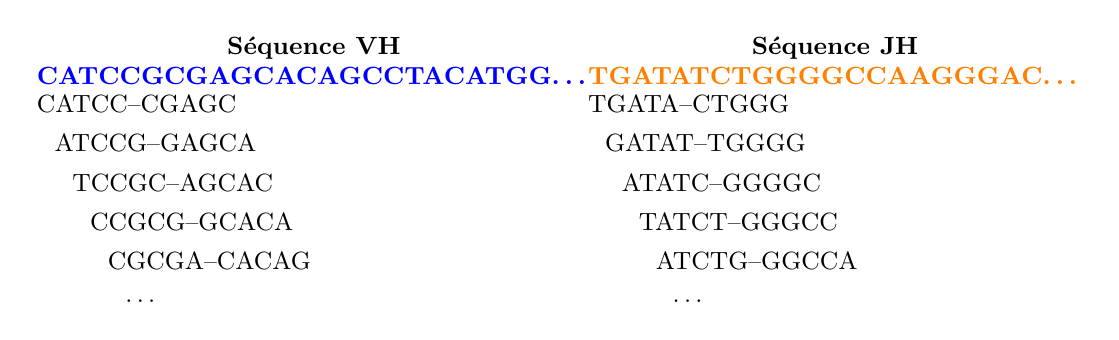
\begin{tikzpicture}[node distance=0cm, thick, font=\small]

    % Séquence VH
    \node[anchor=west] (VH) at (0,0) 
    {\shortstack{\textbf{Séquence VH} \\ \textbf{\textcolor{blue}{CATCCGCGAGCACAGCCTACATGG\dots}}}};
    
    % k-mer espacés séquence VH
    \foreach \i [count=\j from 0] in {
        CATCC--CGAGC,
        ATCCG--GAGCA,
        TCCGC--AGCAC,
        CCGCG--GCACA,
        CGCGA--CACAG,
        \dots
    } {
        \pgfmathsetmacro\xshift{\j*0.225}
        \pgfmathsetmacro\ypos{-0.5*(\j+1.1)}
        \node[anchor=west] at (\xshift,\ypos) {\i};
    }

    % Séquence JH
    \node[anchor=west] (J) at (7,0)
    {\shortstack{\textbf{Séquence JH} \\ \textbf{\textcolor{orange}{TGATATCTGGGGCCAAGGGAC\dots}}}};

    % k-mer espacés séquence JH
    \foreach \i [count=\j from 0] in {
        TGATA--CTGGG,
        GATAT--TGGGG,
        ATATC--GGGGC,
        TATCT--GGGCC,
        ATCTG--GGCCA,
        \dots
    } {
        \pgfmathsetmacro\xshift{7 + \j*0.215}
        \pgfmathsetmacro\ypos{-0.5*(\j+1.1)}
        \node[anchor=west] at (\xshift,\ypos) {\i};
    }

    \end{tikzpicture}
    \caption{Génération de l'index à partir de \textit{k-mer} des séquences germinales 
    \textcolor{blue}{VH (à gauche)} et \textcolor{orange}{JH (à droite)}.}
    \label{fig:index}
\end{figure}

    
La seconde étape consiste à traverser l'ensemble des \textit{reads} en recherchant des fenêtres $\mathbf{w}$ qui recouvrent 
la région \gls{cdr}3 par comparaison de chacun des \textit{k-mer} du \textit{read} à ceux des index générés. Brièvement cette 
approche consiste à conserver les \textit{reads} qui contiennent les \textit{k-mer} d'une séquence V et ceux d'une séquence J, 
de façon à former une une fenêtre $\mathbf{w}$ débutant par les derniers \textit{k-mer} de la séquence V et se terminant 
par les premiers \textit{k-mer} de la séquence J (\autoref{fig:vidjil-algo}).
Cette approche permet une détection rapide (qui croit linéairement avec le nombre de nucléotides), robuste et efficace 
des séquences recombinées. Une fois les fenêtres détectées, \textit{vidjil-algo} regroupe les \textit{reads} en clones, 
puis procède à une segmentation et une annotation des séquences identifiées.

\begin{figure}[H]
    \centering
    \begin{tikzpicture}[node distance=0cm, thick, font=\small]

    % Première ligne
    \node[
        rectangle, 
        fill=blue!30, 
        text width=4cm, 
        align=left,
        minimum width=4cm, 
        minimum height=0.6cm
        ] at (0,0) (v_predicted1) {VVVVVV};

    \node[right=of v_predicted1] (sub) {\textcolor{red}{X}};

    \node[
        rectangle, 
        right=of sub, 
        fill=blue!30, 
        text width=3cm, 
        align=left,
        minimum width=3cm, 
        minimum height=0.6cm
        ] (v_predicted2) {VVVVVVVVVV};

    \node[
        rectangle, 
        right=2cm of v_predicted2, 
        fill=orange!30, 
        text width=5cm, 
        align=left,
        minimum width=5cm, 
        minimum height=0.6cm
        ] (j_predicted) {JJJJJJJJJJJJJJJJJJ};

    % Fenêtre w
    \draw[draw=violet, thick]
        ($(v_predicted2.west)!0.5!(v_predicted2.east) + (0,0.35)$) rectangle
        ($(j_predicted.west)!0.5!(j_predicted.east) + (0,-0.35)$);

    % Annotations
    \node[anchor=north west] at ([yshift=-1pt]v_predicted1.south west) 
        {\scriptsize \textbf{\textcolor{blue}{V prédit}}};

    \draw[thick, blue] ($(v_predicted1.west)+(0,-0.8)$) -- ($(v_predicted2.east)+(0,-0.8)$) 
        node[anchor=north west] at ([yshift=-0.5cm]v_predicted1.south west) 
        {\scriptsize \textcolor{blue}{V réel}};

    \node[anchor=north east] at ([yshift=-1pt]j_predicted.south east) 
        {\scriptsize \textbf{\textcolor{orange}{J prédit}}};

    \draw[thick, orange] ($(j_predicted.west)+(0,-0.8)$) -- ($(j_predicted.east)+(0,-0.8)$) 
        node[anchor=north east] at ([yshift=-0.5cm]j_predicted.south east) 
        {\scriptsize \textcolor{orange}{J réel}};
        
    \node[above=3pt of sub] {\scriptsize \textbf{\textcolor{red}{Substitution}}};

    \node at ($(v_predicted2)!0.5!(j_predicted)+(0,0.6)$) 
        {\scriptsize \textbf{\textcolor{violet}{Fenêtre extraite w}}};

    % Deuxième ligne
    \begin{scope}[yshift=-2cm]

    \node[
        rectangle, 
        fill=blue!30, 
        text width=4cm, 
        align=left,
        minimum width=4cm, 
        minimum height=0.6cm
        ] at (0,0) (v_predicted1b) {VVVVVVVVVVVV};

    \node[
        rectangle, 
        right=-0.5 cm of v_predicted1b, 
        fill=blue!30,
        minimum width=2.5cm, 
        minimum height=0.6cm
        ] (v_predicted2b) {};

    \node[right=of v_predicted2b] (subb) {\textcolor{red}{X}};

    \node[
        rectangle, 
        right=3.7cm of v_predicted2b, 
        fill=orange!30, 
        text width=5cm, 
        align=left,
        minimum width=5cm, 
        minimum height=0.6cm
        ] (j_predictedb) {JJJJJJJJJJJJJJJJJJ};

    % Fenêtre w
    \draw[draw=violet, thick]
        ($(v_predicted2b.west)!0.5!(v_predicted2b.east) + (0,0.35)$) rectangle
        ($(j_predictedb.west)!0.3!(j_predictedb.east) + (0,-0.35)$);

    % Annotations
    \node[anchor=north west] at ([yshift=-1pt]v_predicted1b.south west) 
        {\scriptsize \textbf{\textcolor{blue}{V prédit}}};

    \draw[thick, blue] ($(v_predicted1b.west)+(0,-0.8)$) -- ($(v_predicted2b.east)+(1.7,-0.8)$) 
        node[anchor=north west] at ([yshift=-0.5cm]v_predicted1b.south west) 
        {\scriptsize \textcolor{blue}{V réel}};

    \node[anchor=north east] at ([yshift=-1pt]j_predictedb.south east) 
        {\scriptsize \textbf{\textcolor{orange}{J prédit}}};

    \draw[thick, orange] ($(j_predictedb.west)+(0,-0.8)$) -- ($(j_predictedb.east)+(0,-0.8)$) 
        node[anchor=north east] at ([yshift=-0.5cm]j_predictedb.south east) 
        {\scriptsize \textcolor{orange}{J réel}};
        
    \node[above=3pt of subb] {\scriptsize \textbf{\textcolor{red}{Substitution}}};

    \node at ($(v_predicted2b)!0.6!(j_predictedb)+(0,0.6)$) {\scriptsize \textbf{\textcolor{violet}{Fenêtre extraite w}}};

    \end{scope}

    \end{tikzpicture}
    \caption{
        Illustration du fonctionnement de l'heuristique de \textit{vidjil-algo} sur deux \textit{read} successifs. 
        Adapté de \citeauthor{giraudFastMulticlonalClusterization2014b}. Sur le \textit{read} du haut, \textit{vidjil-algo} 
        prédit avec exactitude les \colorbox{blue!30}{segments V} et \colorbox{orange!30}{J}. Sur le \textit{read} du bas, le 
        \colorbox{blue!30}{segments V} prédit est plus court en raison de la substitution d'un nucléotide. 
    }
    \label{fig:vidjil-algo}
\end{figure}


Les résultats ainsi générés par \textit{vidil-algo} sont rassemblés dans un fichier \textit{.vidjil} au format \gls{json} où 
l'on retrouvera des métadonnées en lien avec l'échantillon analysé et un ensemble de données relatif à chaque clone 
identifié par \textit{vidjil-algo} (\autoref{lst:json-vidjil}).

\begin{lstlisting}[language=json, 
    caption={Extrait d'une sortie de \textit{vidjil-algo}.},
    label={lst:json-vidjil}]
    "clones": [
        {
          "_average_read_length": ["151.80"],
          "_coverage_info": [ "132 bp (86% of 151.8 bp)"],
          "germline": "IGH",
          "id": "GGGGATAAATTACGATTTTTGGAGTGGTTATTAT...GGGGGTT",
          "name": "IGHV1-8*01 0/CGGGGGGATAA/2 IGHD3-3*01 0/GGTATGGGGGGTTTTAG/7 IGHJ4*02",
          "reads": [498126],
          ...
        }
    ]
\end{lstlisting}

\vspace{1em}

En parallèle, \textit{Vidjil} désigne également l'application web (\href{https://app.vidjil.org/}{démo publique accessible ici}) 
permettant de visualiser et de manipuler les résultats produits par \textit{vidjil-algo}. 
Elle prend également en charge la création et la gestion des comptes utilisateurs, des profils patients, etc. (\autoref{fig:vidjil-web}). 
L'application est développée côté serveur en \texttt{Python}, à l'aide du \textit{framework} \href{https://py4web.com}{\texttt{py4web}} 
(anciennement \texttt{web2py}), et côté client en \texttt{JavaScript}. La base de données utilisée est \texttt{MySQL}, 
le tout étant orchestré via le déploiement de conteneurs \texttt{Docker}.

\begin{figure}[H]
    \centering
    \includegraphics[width=0.9\textwidth]{images/vidjil-web.png}
    \caption{Interface de la plateforme web \textit{Vidjil}. 
    Liste des clones identifiés à gauche, visualisation de la cinétique des clones en haut à gauche, 
    familles \gls{vdj} en bas à droite, et séquences des clones sélectionnés en bas.}
    \label{fig:vidjil-web}
\end{figure}

\section{Applications en oncohématologie}

L'analyse du répertoire des gènes \gls{vdj} est particulièrement utile en oncohématologie, 
où la quasi unicité de chaque réarrangement \gls{vdj} peut servir de marqueur clonal hautement 
spécifique des cellules tumorales et ainsi permettre leur détection et leur suivi \cite{hultcrantzBaselineVDJClonotype2020}.

\vspace{1em}
 
Avant toute chose, il peut être utile de dresser un panorama rapide des hémopathies malignes afin de 
mieux comprendre l'importance de l'analyse du répertoire des gènes \gls{vdj} dans certaines situations.  
Ces pathologies regroupent ce qu'on appelle communément les « cancers du sang » et peuvent se séparer selon
leur origine en quatre grandes catégories. Une première séparation peut être établie entre les hémopathies 
myéloïdes et lymphoïdes selon l'origine des cellules. Brièvement, les cellules du sang et de la moelle sont soit de 
lignée lymphoïde pour les lymphocytes (B, T, NK et autres non conventionnels) et précurseurs, soit de lignée myéloïde 
pour le reste des cellules (hématies, plaquettes, polynucléaires, monocytes) et leurs précurseurs. Une seconde séparation 
est établie selon la maturité des cellules : on parle alors de \glspl{lam} et de \glspl{lal} lorsque la cellule 
tumorale dérive d'un précurseur, et de \glspl{smp} et de \glspl{slp}/\glspl{lnh} lorsque la cellule est mature 
\cite{alaggio5thEditionWorld2022a, khoury5thEditionWorld2022}.

\begin{figure}[H]
    \centering
    \begin{tikzpicture}[
        node distance=1cm and 3mm,
        every node/.style={
            draw,
            align=center,
            font=\scriptsize,
            text width=1.6cm,
            minimum height=0.7cm
        },
        lymphprecursor/.style={fill=Purple!20},
        lymphmature/.style={fill=Purple!60},
        lymphmature2/.style={fill=Purple},
        myeloprecursor/.style={fill=Rhodamine!30},
        myelomature/.style={fill=Rhodamine!70},
        img/.style={draw=none, minimum height=0mm, inner sep=0pt}
    ]

    % Root node
    \node (csh) [text width=4cm] {Cellule souche  hématopoïétique multipotente (CSH)};

    % Myeloid branch
    \node (myeloid) [below left=of csh, myeloprecursor] {Progéniteur  myéloïde};

    \node (erytho) [below=of myeloid, myeloprecursor] {Érythroblaste};
    \node (megaka) [left=of erytho, myeloprecursor] {Mégacaryocyte};
    \node (monoblast) [right=of erytho, myeloprecursor] {Monoblaste};
    \node (myeloblast) [right=of monoblast, myeloprecursor] {Myéloblaste};

    \node (plaq) [below=of megaka, myelomature] {Plaquette};
    \node (gr)   [below=of erytho, myelomature] {Globule  rouge};

    \node (mono)  [below=of monoblast, myelomature] {Monocyte};
    \node (eosino) [below=3.5cm of myeloblast, myelomature] {Granulocyte  éosinophile};
    \node (neutro) [right=of eosino, myelomature] {Granulocyte  neutrophile};
    \node (baso)   [right=of neutro, myelomature] {Granulocyte  basophile};


    % Lymphoid branch
    \node (lymphoid) [right=8cm of myeloid, lymphprecursor] {Progéniteur  lymphoïde};

    \node (bcell) [below=of lymphoid, lymphmature] {Lymphocyte B};
    \node (tcell) [right=of bcell, lymphmature] {Lymphocyte T};
    \node (nkcell) [left=of bcell, lymphmature] {Cellule NK};
    \node (plasmocyte) [below=of bcell, lymphmature2] {Plasmocyte};

    % Images
    \node[img, below=2pt of plaq] {\includegraphics[width=1.5cm]{images/plt.png}};
    \node[img, below=2pt of gr] {\includegraphics[width=1.5cm]{images/gr.png}};
    \node[img, below=2pt of mono] {\includegraphics[width=1.5cm]{images/monocyte.png}};
    \node[img, below=2pt of eosino] {\includegraphics[width=1.5cm]{images/pne.png}};
    \node[img, below=2pt of neutro] {\includegraphics[width=1.5cm]{images/pnn.png}};
    \node[img, below=2pt of baso] {\includegraphics[width=1.5cm]{images/pnb.png}};
    \node[img, below right=1.5pt of bcell] {\includegraphics[width=1.5cm]{images/lympho.png}};
    \node[img, below=2pt of plasmocyte] {\includegraphics[width=1.5cm]{images/plasmo.png}};
    \node[img, below=5pt of nkcell] {\includegraphics[width=1.5cm]{images/lynk.png}};

    % Disease boxes
    \node[
        fit=(myeloid)(erytho)(monoblast)(myeloblast), 
        draw=Rhodamine!40, 
        dotted, 
        ultra thick, 
        inner sep=5pt, 
        label=above right:{\textbf{\textcolor{Rhodamine!40}{LAM}}}
    ] {};

    \node[
        fit=(baso)(eosino)(neutro), 
        draw=Rhodamine, 
        dotted, 
        ultra thick, 
        inner sep=5pt, 
        label=above left:{\textbf{\textcolor{Rhodamine}{LMC}}}
    ] {};

    \node[
        fit=(plaq)(gr)(mono), 
        draw=Rhodamine, 
        dotted, 
        ultra thick, 
        inner sep=5pt, 
        label=above right:{\textbf{\textcolor{Rhodamine}{SMP}}}
    ] {};

    \draw[
    draw=Purple!40, 
    dotted, 
    ultra thick, 
    ]
    ($(lymphoid.south west) + (-3pt,-3pt)$)
    rectangle
    ($(lymphoid.north east) + (3pt,3pt)$);

    \node[draw=none, thick, text=Purple!40] 
    at ($(lymphoid.north) + (0,0.5cm)$) 
    {\textbf{LAL}};

    \node[
        fit=(nkcell)(bcell)(tcell), 
        draw=Purple!60, 
        dotted, 
        ultra thick, 
        inner sep=5pt, 
        label={[xshift=-15pt]above left:{\textbf{\textcolor{Purple!60}{SLP/LNH}}}}
    ] {};

    \draw[
        draw=Purple!60, 
        dotted, 
        ultra thick, 
        ]
        ($(bcell.south west) + (-3pt,-10pt)$)
        rectangle
        ($(bcell.north east) + (3pt,10pt)$);
    
    \node[draw=none, thick, text=Purple!60] 
    at ($(bcell.north) + (0.5,0.6cm)$) 
    {\textbf{LLC}};

    \draw[
        draw=Purple,
        line width=3pt,
        line cap=rect,
        dash pattern=on 0pt off 6pt,
    ]
        ($(plasmocyte.south west) + (-3pt,-3pt)$)
        rectangle
        ($(plasmocyte.north east) + (3pt,3pt)$);    

    \node[draw=none, thick, text=Purple] 
    at ($(plasmocyte.west) + (-0.5,0cm)$) 
    {\textbf{MM}};

    % Connections
    \draw[-] (csh) -- (myeloid);
    \draw[-] (csh) -- (lymphoid);

    \draw[-] (myeloid) -- (erytho);
    \draw[-] (myeloid) -- (megaka);
    \draw[-] (myeloid) -- (myeloblast);
    \draw[-] (myeloid) -- (monoblast);

    \draw[-] (megaka) -- (plaq);
    \draw[-] (erytho) -- (gr);
    \draw[-] (myeloblast) -- (neutro);
    \draw[-] (myeloblast) -- (eosino);
    \draw[-] (myeloblast) -- (baso);
    \draw[-] (monoblast) -- (mono);

    \draw[-] (lymphoid) -- (bcell);
    \draw[-] (lymphoid) -- (tcell);
    \draw[-] (lymphoid) -- (nkcell);
    \draw[-] (bcell) -- (plasmocyte);

    \end{tikzpicture}
    \caption{
        Classification des hémopathies malignes selon la lignée cellulaire d'origine 
        (\colorbox{Rhodamine!60}{myéloïde} à gauche ou \colorbox{Purple!60}{lymphoïde} à droite) 
        et le stade de maturation des cellules (\colorbox{Gray!20}{immature} en haut et \colorbox{Gray!70}{mature} en bas).
        LAM : leucémies aiguës myéloïdes, LAL : leucémies aiguës lymphoblastiques, SMP : syndromes myéloprolifératifs, 
        LMC : leucémie myéloïde chronique, SLP : syndromes lymphoprolifératifs, LNH : lymphomes non hodgkiniens, 
        LLC : leucémie lymphoïde chronique, MM : myélome multiple.
    }
    \label{fig:hemopathies}
\end{figure}


Dès lors \textit{Vidjil} trouve son utilité dans les hémopathies lymphoïdes, principalement dans les \glspl{lal} et les 
\glspl{llc} où il permet l'identification des réarrangements \gls{vdj} des \glspl{ig} et des \glspl{tcr} à des fins diverses.
Par exemple, dans les \glspl{llc} il permet d'identifier et d'annoter le segment V du réarrangement \gls{igh} du clone tumoral, pour 
ensuite étudier le taux de mutations face aux séquences germinales, servant de marqueur pronostique fort de la pathologie
\cite{crombieIGHVMutationalStatus2017}.

\vspace{1em}

Dans le cadre de ce travail, nous nous sommes intéréssés à une pathologie en particulier, le \gls{mm} qu'il est possible 
de rattacher au groupes des hémopathies lymphoïdes matures. Cette pathologie 

\section{Maladie résiduelle et ADNc}

\section{Problématique et objectifs}
